\documentclass[a4paper,10pt]{article}
%\documentclass[a4paper,10pt]{scrartcl}

\usepackage{amsmath}% $ \implies $
\usepackage{amssymb}% \blacksquare
\usepackage{tikz-qtree}% tikzpicture
\usepackage[utf8]{inputenc}

\title{Symbolic Logic and Mechanical Theorem Proving -- Respostas}
\author{Ricardo Fantin da Costa}
\date{23-09-2018}

\pdfinfo{%
  /Title    (Symbolic Logic and Mechanical Theorem Proving -- Respostas)
  /Author   (Ricardo Fantin da Costa)
  /Creator  ()
  /Producer ()
  /Subject  ()
  /Keywords (Respostas)
}

\begin{document}
\maketitle

\section{Exercícios Recomendados}
A lista de exercícios recomendados pelo professor está abaixo. Os sublinhados são fortemente recomendados.

\begin{itemize}
 \item Cap. 2: 3, 4, 6, 7, 8, \underline{9}, 10, 14
 \item Cap. 3: 5, \underline{6}, 7, 8, \underline{9}
 \item Cap. 4: \underline{1}, \underline{5}, 8, \underline{9}, 10, 11, 12, 13, \underline{14}
 \item Cap. 5: 1, 2, 3, \underline{6}, 7 \underline{8}, 9, \underline{10}, \underline{12}, \underline{13}, \underline{14}
\end{itemize}

Exercícios que começam com * estão incluídos nessa lista, porém foram mesmo assim.

\section{The Propositional Logic}
3. Complete the following truth table (Table 2.11 -- Tabela~\ref{tab:pergunta2.3}) of the formula

\begin{equation}
 (\sim P \vee Q) \wedge (\sim(P \vee \sim Q))
\end{equation}

\begin{table}
 \begin{tabular}{cccccccc}
  \hline
  P & Q & $\sim P$ & $\sim Q$ & $\sim P \vee Q$ & $P \wedge \vee Q$ & $\sim(P \wedge \sim Q)$ & $(\sim P \vee Q) \wedge (\sim(P \vee \sim Q))$ \\
  \hline
  T & T & & & & & & \\
  T & F & & & & & & \\
  F & T & & & & & & \\
  F & F & & & & & & \\
  \hline
 \end{tabular}
 \caption{Tabela da pergunta 3 do capítulo 2.}
 \label{tab:pergunta2.3}
\end{table}

Resposta na Tabela~\ref{tab:resposta2.3}.

\begin{table}
 \begin{tabular}{cccccccc}
  \hline
  P & Q & $\sim P$ & $\sim Q$ & $\sim P \vee Q$ & $P \wedge \sim Q$ & $\sim(P \wedge \sim Q)$ & $(\sim P \vee Q) \wedge (\sim(P \wedge \sim Q))$ \\
  \hline
  T & T & F & F & T & F & T & T \\
  T & F & F & T & F & T & F & F \\
  F & T & T & F & T & F & T & T \\
  F & F & T & T & T & F & T & T \\
  \hline
 \end{tabular}
 \caption{Tabela da resposta 3 do capítulo 2.}
 \label{tab:resposta2.3}
\end{table}

4. For each of the following formulas, determine whether it is valid, invalid, inconsistent, consistent, or some combination of these.
\begin{enumerate}
 \item[(a)] $ \sim(\sim P) \implies P $ \newline
válido, consistente
 \item[(b)] $ P \implies (P \wedge Q) $ \newline
inválido, consistente
 \item[(c)] $ \sim(P \vee Q) \vee \sim Q $ \newline
inválido, consistente
 \item[(d)] $ (P \vee Q) \implies P $ \newline
inválido, consistente
 \item[(e)] $ (P \implies Q) \implies ( \sim Q \implies \sim P) $ \newline
inválido, consistente
 \item[(f)] $ (P \implies Q) \implies ( Q \implies P) $ \newline
inválido, consistente
 \item[(g)] $ P \vee (P \implies Q) $ \newline
válido, consistente
 \item[(h)] $ (P \wedge (Q \implies P)) \implies P $ \newline
válido, consistente
 \item[(i)] $ P \vee (Q \implies \sim P) $ \newline
válido, consistente
 \item[(j)] $ (P \vee \sim Q) \wedge (\sim P \vee Q) $ \newline
inválido, consistente
 \item[(k)] $ (\sim P \wedge (\sim (P \implies Q)) $ \newline
inválido, consistente
 \item[(l)] $ P \implies \sim P $ \newline
inválido, consistente
 \item[(m)] $ \sim P \implies P $ \newline
inválido, consistente
\end{enumerate}

6. Transform the following into disjunctive normal forms.

\begin{enumerate}
 \item[(a)] $ (\sim P \wedge Q) \implies R $ \newline
$P \vee \sim Q \vee R$
 \item[(b)] $ P \implies \left( ( Q \wedge R) \implies S \right)$ \newline
$ \sim P \vee \sim Q \vee \sim R \vee S $
 \item[(c)] $ \sim (P \vee \sim Q) \wedge (S \implies T) $ \newline
$ \sim P \wedge \sim Q \wedge (\sim S \vee T) $
 \item[(d)] $ (P \implies Q) \implies R $ \newline
$ P \wedge \sim Q \vee R $
 \item[(e)] $ \sim (P \wedge Q) \wedge (P \vee Q) $. \newline
$ (\sim P \vee \sim Q) \wedge (P \vee Q) $
\end{enumerate}

7. Transform the following into conjunctive normal forms
\begin{itemize}
 \item[(a)] $ P \vee (\sim P \wedge Q \wedge R) $ \newline
$(P \vee Q) \wedge (P \vee R) $
 \item[(b)] $ \sim (P \implies Q) \vee (P \vee Q) $ \newline
$ P \vee Q $
 \item[(c)] $ \sim (P \implies Q) $ \newline
$ P \wedge \sim Q $
 \item[(d)] $ (P \implies Q) \implies R $ \newline
$ (P \vee R) \wedge (\sim Q \vee R) $
 \item[(e)] $ (\sim P \wedge Q) \vee (P \wedge \sim Q) $ \newline
$ (P \vee Q) \wedge (\sim P \vee \sim Q) $
\end{itemize}

8. Is it possible to have a formula that is in conjunctive normal form as well as disjunctive normal form? If yes, give an example.

Sim, possíveis fórmulas: P, $ P \vee Q $ ou $ P \wedge Q $.

\underline{9.} Verify each of the following pairs of equivalent formulas by transforming formulas on both sides of the sigh = into the same normal form.
\begin{itemize}
 \item[(a)] $ P \wedge P = P $, and $ P \vee P = P $ \newline
P = P e P = P
 \item[(b)] $ (P \implies Q) \wedge (P \implies R) = (P \implies (Q \wedge R)) $ \newline
$ (\sim P \vee Q) \wedge (\sim P \vee R) $
 \item[(c)] $ (P \implies Q) \implies (P \wedge Q) = (\sim P \implies Q) \wedge (Q \implies P) $ \newline
As fórmulas não representam o mesmo valor verdade. A primeira fórmula é igual a P e a segunda é $ \sim Q \vee P $.
 \item[(d)] $ P \wedge Q \wedge (\sim P \vee \sim Q) = \sim P \wedge \sim Q \wedge (P \vee Q) $ \newline
$ \square $
 \item[(e)] $ P \vee (P \implies (P \wedge Q)) = \sim P \vee \sim Q \vee (P \wedge Q) $. \newline
$ \blacksquare $
\end{itemize}

10. Prove that $ (\sim Q \implies \sim P) $ is logical consequence of $(P \implies Q) $ .

$P \implies Q$

$\sim P \vee Q$

$Q \vee \sim P$

$\sim Q \implies \sim P$

14. Show that Q is a logical consequence of $ (P \implies Q) $ and P. This is related to the so-called modus ponens rule.

Dado que P tem valor 1, o  valor de $ (P \implies Q) $ equivale ao valor de Q. Desta forma P e $ (P \implies Q) $ equivale a Q.

\section{The First-Order Logic}
1. Let P(x) and Q(x) represent ``x is a rational number 11 and ``x is a real number, '' respectively. Symbolize the following sentences:
\begin{itemize}
 \item[1.1] Every rational number is a real number. \newline
$ (\forall x) P(x) \implies Q(x) $
 \item[1.2] Some real numbers are rational numbers. \newline
$ (\exists x) Q(x) \implies P(x) $ \newline
ou \newline
$ (\exists x) Q(x) \wedge P(x) $
 \item[1.3] Not every real number is a rational number. \newline
$ (\exists x) Q(x) \wedge P(x) $
\end{itemize}

5. For the following interpretation (D = \{a,b\}), (Tabela~\ref{tab:pergunta3.5})
\begin{table}
 \centering
 \begin{tabular}{cccc}
  \hline
  P(a,a) & P(a,b) & P(b,a) & P(b,b) \\ \hline
  T & F & F & T \\ \hline
 \end{tabular}
 \label{tab:pergunta3.5}
 \caption{Interpretação proposta no enunciado da questão 3.5.}
\end{table}
, determine the truth value of the following formulas:
\begin{itemize}
 \item[(a)] $ (\forall x) (\exists y) P(x,y) $ \newline
$ \blacksquare $
 \item[(b)] $ (\forall x) (\forall y) P(x,y) $ \newline
$ \square $
 \item[(c)] $ (\exists x) (\forall y) P(x,y) $ \newline
$ \square $
 \item[(d)] $ (\exists y) \sim P(a,y) $ \newline
$ \blacksquare $
 \item[(e)] $ (\forall x) (\forall y) (P(x,y) \implies P(y,x)) $ \newline
$ \blacksquare $
 \item[(f)] $ (\forall x) P(x,x) $ \newline
$ \blacksquare $
\end{itemize}

\underline{6.} Consider the following formula:

$ A: (\exists x) P(x) \implies (\forall x) P(x). $

a. Prove that this formula is always true if the domain D contains only one element.

Com apenas um elemento no domínio, por exemplo a, só existe um valor verdade para P(a). Sendo F ou T, $ F \implies F $ ou $ T \implies T $ tem como valor verdade T.

b. Let D = \{a,b\}. Find an interpretation over D in which A is evaluated to F.

Sendo P(a) = T e P(b) = F, a fórmula $ P(a) \implies P(b) $ resulta em F.

7. Consider the following interpretation:

Domain: D = \{1,2\}.

Assignment of constants a and b (Tabela~\ref{tab:pergunta7a}):

\begin{table}
 \centering
 \begin{tabular}{cc}
  \hline
  a & b \\ \hline
  1 & 2 \\ \hline
 \end{tabular}
 \caption{Valores das constantes a e b pro exercício 7.}
 \label{tab:pergunta7a}
\end{table}

Assignment for function f (Tabela~\ref{tab:pergunta7b}):

\begin{table}
 \centering
 \begin{tabular}{cc}
  \hline
  f(1) & f(2) \\ \hline
  2 & 1 \\ \hline
 \end{tabular}
 \caption{Valores da função \texttt{f()} pro exercício 7.}
 \label{tab:pergunta7b}
\end{table}

Assignment for predicate P (Tabela~\ref{tab:pergunta7c}):

\begin{table}
 \centering
 \begin{tabular}{cccc}
  \hline
  P(1,1) & P(1,2) & P(2,1) & P(2,2) \\ \hline
  T & T & F & F \\ \hline
 \end{tabular}
 \caption{Valores do predicado \texttt{P()} pro exercício 7.}
 \label{tab:pergunta7c}
\end{table}

Evaluate the truth value of the following formulas in the above interpretation:
\begin{itemize}
 \item[(1)] $ P(a, f(a)) \wedge P(b, f(b)) $ \newline
$ \square $
 \item[(2)] $ (\forall x) (\exists y) P(y,x) $ \newline
$ \blacksquare $
 \item[(3)] $ (\forall x) (\forall y) (P(x,y) \implies P(f(x),f(y))) $. \newline
$ \blacksquare $
\end{itemize}

8. Let F1 and F2 be as follows:

$ F_1: (\forall x) (P(x) \implies Q(x)) $

$ F_2: \sim Q(a). $

Prove that $\sim P(a)$ is a logical consequence of F1 and F2.

De $F_1$ com $ S = \{ a \diagup x\} $ obtêm-se $ P(a) \implies Q(a) $. Como deseja-se provar $\sim P(a)$, adiciona-se $ P(a) $ e a cláusula vazia é buscada. De P(a) e $ P(a) \implies Q(a) $, com o modus pones obtêm-se Q(a). Unindo as clausulas Q(a) e $ F_2: \sim Q(a) $ chega-se a cláusula vazia.

\underline{9.} Transform the following formulas into prenex normal forms:
\begin{itemize}
 \item[(1)] $ (\forall x) (P(x) \implies (\exists y) Q(x,y)) $ \newline
$(\forall x) (\exists y) P(x) \implies Q(x, y) $
 \item[(2)] $ (\exists x) (\sim((\exists y)P(x,y)) \implies ((\exists z) Q(z) \implies R(x))) $ \newline
$(\exists x)(\exists y)(\forall z) \sim P(x,y) \vee \sim Q(z) \vee R(x) $
 \item[(3)] $ (\forall x)(\forall y)((\exists z) P(x,y,x) \wedge((\exists u) Q(x,u) \implies (\exists v) Q(y,v))) $. \newline
$ (\forall x)(\forall y)(\exists z)(\forall u)(\exists v)(P(x,y,x) \wedge (\sim (Q(x,u) \vee Q(y,v)))) $
\end{itemize}

\section{Herbrand's Theorem}

\underline{1.} Find a standard form from for each of the following formulas:
\begin{itemize}
 \item[(a)] $ \sim ((\forall x) P(x) \implies (\exists y) (\forall z) Q(y,z)) $ \newline
$ P(x) \wedge \sim Q(y, f(x, y)) $
 \item[(b)] $ (\forall x)((\sim E(x,0)\implies((\exists y)(E(y,g(x)) \wedge (\forall z)(E(z,g(x)) \implies E(y,z))))) $ \newline
$ E(x,0) \vee (E(f(x),g(x)) \wedge ( (\sim E(z,g(x)) \vee E(f(x),z))) )$
 \item[(c)] $ \sim((\forall x)P(x) \implies(\exists y)P(y)) $.
 \newline
$ P(x) \vee P(f(x)) $
\end{itemize}

\underline{5.} Let S = \{P(f(x),a,g(f(x),b))\}.
\begin{itemize}
 \item[(1)] Find H0 and H1. \newline
$ H_0 = \{ a, b \} $ \newline
$ H_1 = \{ a, b, f(a), f(b), g(a, a), g(a, b), g(b, a), g(b, b) \} $
 \item[(2)] Find all the ground instances of S over H0. \newline
$ P(a), P(b), g(f(a)), g(f(b)) $
 \item[(3)] Find all the ground instances of S over H1. \newline
$ P(a), P(b), P(f(a)), P(f(b)), P(g(a,a)), P(g(a,b)), P(g(b,a)), P(g(b,b)),\\
g(f(a),b), g(f(b),b), g(f(f(a)),b), g(f(f(b)),b), g(f(g(a,a)),b),\\
g(f(g(a,b)),b),g(f(g(b,a)),b), g(f(g(b,b)),b)$
\end{itemize}

8. Consider the following clause C and interpreation I:

$ C: P(x) \vee Q(x,f(x)) $

$I:\\
\{ \sim P(a), \sim P(f(a)), \sim P(f(f(a))), ...,\\
\sim Q(a,a), Q(a, f(a)), \sim Q(a,f(f(a))), ...,\\
\sim Q(f(a,a),Q(f(a),f(a)), \sim Q(f(a), f(f(a))), ... \}.$

Does I satisfy C?

Não. S' = \{P(a), Q(a, f(a))\}.

\underline{9.} Consider the following set S of clauses:

\[
S =	\begin{cases}
		P(x) \\
		Q(f(y)).
	\end{cases}
\]

Let an interpretation I be defined as below:

$I =\\
\{P(a), P(f(a)), P(f(f(a))), ...,\\
Q(a), \sim Q(f(a)), Q(f(f(a))), ...\}.
$

Does I satisfy S?

Não. S' = \{P(a), Q(f(a))\}.

10. Consider $ S = \{P(x), \sim P(f(y))\} $.

\begin{itemize}
 \item[1.] Give H0, H1, H2, and H3 of S. \newline
$ H_0 = \{a\} $ \newline
$ H_1 = \{a, f(a)\} $ \newline
$ H_2 = \{a, f(a), f(f(a))\} $ \newline
$ H_3 = \{a, f(a), f(f(a)), f(f(f(a)))\} $
 \item[2.] Is it possible to find an interpreation that satisfies S? If yes, give one. If no, why?

Não existe interpretação que satisfaz S. Os dois primeiros termos da interpretação devem ser $I = \{ P(a), \sim P(f(a)) \}$. Considerando x = f(a), a fórmula já não seria satisfeita.
\end{itemize}

11. Let $ S = \{P, \sim P \vee Q, \sim Q\} $. Give a closed semantic tree of S.

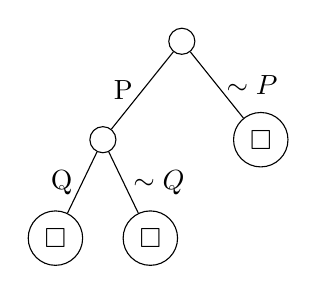
\begin{tikzpicture}[every tree node/.style={draw,circle},
   level distance=1.25cm,sibling distance=.5cm, 
   edge from parent path={(\tikzparentnode) -- (\tikzchildnode)}]
\Tree [.\node { };
        \edge node[left] {P};
        [.{ } 
          \edge node[left] {Q};
          [.{$ \square $} ]
          \edge node[right] {$\sim Q$};
          [.{$ \square $} ]
        ]
        \edge node[right] {$\sim P$};
        [.{$ \square $} ]
      ]
\end{tikzpicture}

12. Consider $ S = \{P(x), \sim P(x) \vee Q(x,a), \sim Q(y,a)\} $.
\begin{itemize}
 \item[(a)] Give the atom set of S. \newline
S = \{P(a), Q(a,a)\}
 \item[(b)] Give a complete semantic tree of S. \newline
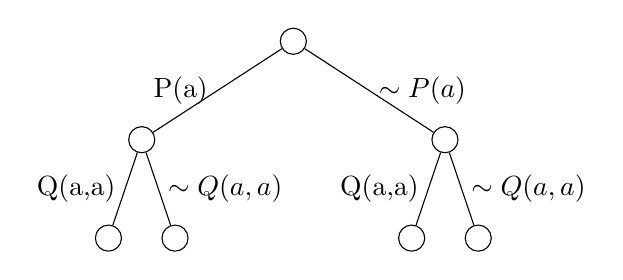
\begin{tikzpicture}[every tree node/.style={draw,circle},
   level distance=1.25cm,sibling distance=.5cm, 
   edge from parent path={(\tikzparentnode) -- (\tikzchildnode)}]
\Tree [.\node { };
        \edge node[left] {P(a)};
        [.{ } 
          \edge node[left] {Q(a,a)};
          [.{ } ]
          \edge node[right] {$\sim Q(a,a)$};
          [.{ } ]
        ]
        \edge node[right] {$\sim P(a)$};
        [.{ } 
          \edge node[left] {Q(a,a)};
          [.{ } ]
          \edge node[right] {$\sim Q(a,a)$};
          [.{ } ]
        ]
      ]
\end{tikzpicture}
 \item[(c)] Give a closed semantic tree of S. \newline
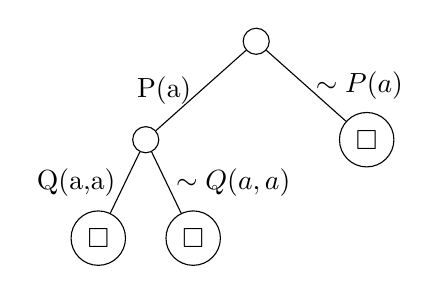
\begin{tikzpicture}[every tree node/.style={draw,circle},
   level distance=1.25cm,sibling distance=.5cm, 
   edge from parent path={(\tikzparentnode) -- (\tikzchildnode)}]
\Tree [.\node { };
        \edge node[left] {P(a)};
        [.{ }
          \edge node[left] {Q(a,a)};
          [.{$\square$} ]
          \edge node[right] {$\sim Q(a,a)$};
          [.{$\square$} ]
        ]
        \edge node[right] {$\sim P(a)$};
        [.{$\square$} ]
      ]
\end{tikzpicture}
\end{itemize}

13. Consider $ S = \{P(x,a,g(x,b)), \sim P(f(y),z,g(f(a),b))\} $. Find an unsatisfiable set S' of ground instances of clauses in S.

$ S' = \{ P(f(y),a,g(f(a),b)), \sim P(f(y),a,g(f(a),b)) \} $

\underline{14.} Let $ S = \{P(x),Q(x,f(x)) \vee \sim P(x), \sim Q(g(y),z)\} $. Find an unsatisfiable set S' of ground instances of clauses in S.

$ S' = \{ P(x), Q(g(y),f(g(y)))\vee \sim P(x), \sim Q(g(y),f(g(y)))\} $
\section{The Resolution Principles}

1. Prove the following set of clauses is unsatisfiable by resolution:

$ P \vee Q \vee R, \sim P \vee R, \sim Q, \sim R $.

\begin{itemize}
 \item[(1)] $ P \vee Q \vee R $
 \item[(2)] $ \sim P \vee R $
 \item[(3)] $ \sim Q $
 \item[(4)] $ \sim R $
 \item[(5)] $ P $ de (1), (3) e (4)
 \item[(6)] $ R $ de (2) e (5)
 \item[(7)] $ \square $ de (4) e (6)
\end{itemize}

2. For the set $ S = \{P\vee Q, \sim Q \vee R, \sim P \vee Q, \sim R\} $ derive an empty clause from S by resolution.

\begin{itemize}
 \item[(1)] $ P \vee Q $
 \item[(2)] $ \sim Q \vee R $
 \item[(3)] $ \sim P \vee Q $
 \item[(4)] $ \sim R $
 \item[(5)] $ \sim Q $ de (2) e (4)
 \item[(6)] $ Q $ de (1) e (3)
 \item[(7)] $ \square $ de (5) e (6)
\end{itemize}

3. Let $ \Theta = \{ a\diagup x, b\diagup y, g(x,y)\diagup z \} $ be a substituion and E = P(h(x),z). Find $E\Theta$.

$E\Theta = P(h(a), g(a,b)) $

\underline{6.}Determine whether each of the following sets is unifiable. If yes, obtain a most general unifies.
\begin{itemize}
 \item[(1)] W = \{Q(a), Q(b)\} \newline
Não unificável.
 \item[(2)] W = \{Q(a,x),Q(a,a)\} \newline
$ S = \{ a \diagup x \} $ \newline
W = Q(a, a)
 \item[(3)] W = \{Q(a,x,f(x)),Q(a,y,y)\} \newline
Não unificável.
 \item[(4)] W = \{Q(x,y,z),Q(u,h(v,v),u)\} \newline
$ S = \{u \diagup x, y \diagup h(v,v), z \diagup u \} $ \newline
W = Q(z,y,z)
 \item[(5)] $ W = \{P(x_1,g(x_1),x_2,h(x_1,x_2),x_3,k(x_1,x_2,x_3)), P(y_1,y_2,e(y_2),y_3,f(y_2,y_3),y_4)\} $. \newline
$ S = \{ x_1 \diagup y_1, g(x_1) \diagup y_2, e(g(x_1)) \diagup x_2, h(x_1, e(g(x_1))) \diagup y_3, f(g(x_1), h(x_1,e(g(x_1)))) \diagup x_3,\newline k(x_1, e(g(x)), f(g(x)), h(x_1,e(g(x_1)))) \diagup y_4 \} $\newline
$ W = P(x_1, g(x_1), e(g(x_1)), h(x_1, e(g(x))), h(x_1,e(g(x_1))) , k(x_1,e(g(x_1))))$
\end{itemize}

7. Determine whether the following clauses have factors. If yes, give the factors.
\begin{itemize}
 \item[(1)] $ P(x) \vee Q(y) \vee P(f(x)) $ \newline
$ \sigma = \{x \diagup f(x) \} \\
(1)\sigma = P(x) \vee Q(y) $
 \item[(2)] $ P(x) \vee P(a) \vee Q(f(x)) \vee Q(f(a)) $ \newline
$ \sigma = \{x \diagup a \} \\
(2)\sigma = P(x) \vee Q(f(x)) $
 \item[(3)] $ P(x, y) \vee P(a, f(a)) $ \newline
$ \sigma = \{ x \diagup a, y \diagup f(a) \} \\
(3)\sigma = P(x, y) $
 \item[(4)] $ P(a) \vee P(b) \vee P(x) $ \newline
$ \sigma = \{x \diagup a, x \diagup b \} \\
(4)\sigma = P(x)$
 \item[(5)] $ P(x) \vee P(f(y)) \vee Q(x,y) $. \newline
Não possui.
\end{itemize}

\underline{8.} Find all possible resolvents (if any) of the following pairs of clauses:
\begin{itemize}
 \item[(1)] $ C = \sim P(x) \vee Q(x,b) $, $ D = P(a) \vee Q(a,b) $ \newline
Q(a,b)
 \item[(2)] $ C = \sim P(x) \vee Q(x,x) $, $ D = \sim Q (a,f(a)) $ \newline
Não existe.
 \item[(3)] $ C = \sim P(x,y,u) \vee \sim P(y,z,v) \vee \sim P(x,v,w) \vee P(u,z,w) $, $ D = P(g(x,y),x,y) $ \newline
Não existe.
 \item[(4)] $ C = \sim P(v,z,v) \vee P(w,z,w) $, $ D = P(w,h(x,x),w) $. \newline
P(w,z,w)
\end{itemize}

9. Reconsider Example 2.13 in Section 2.6. This time show that $H_2CO_3$ can be made by resolution.

Primeiro nega-se a consequência $H_2CO_3$ para obter $ \sim H_2CO_3 $. Remove-se as consequências $ (MgO \wedge H_2) \implies (Mg \wedge H_2O) \equiv \sim MgO \vee \sim H_2 \vee (Mg \wedge H_2O)$, $ C \wedge O_2 \implies CO_2 \equiv \sim C \vee \sim O_2 \vee CO_2$ e $ CO_2 \wedge H_2O \implies H_2CO_3 \equiv \sim CO_2 \vee \sim H_2O \vee H_2CO_3$.

\begin{itemize}
 \item[(1)] $ \sim MgO \vee \sim H_2 \vee (Mg \wedge H_2O) $
 \item[(2)] $ \sim C \vee \sim O_2 \vee CO_2 $
 \item[(3)] $ \sim CO_2 \vee \sim H_2O \vee H_2CO_3 $
 \item[(4)] MgO
 \item[(5)] $ H_2 $
 \item[(6)] $ O_2 $
 \item[(7)] C
 \item[(8)] $ \sim H_2CO_3 $
 \item[(9)] $ \sim CO_2 \vee \sim H_2O $ de (3) e (8)
 \item[(10)] $ \sim C \vee \sim O_2 \vee \sim H_2O $ de (2) e (9)
 \item[(11)] $ \sim H_2O $ de (6), (7) e (10)
 \item[(12)] $ Mg \wedge H_2O $ de (1), (4) e (5)
 \item[(13)] $ H_2O $ de (12)
 \item[(14)] $ \square $ de (11) e (13)
\end{itemize}

\underline{10.} In Exercise 14 of Chapter 2, you were asked to show that Q is a logical consequence of P and $ P \implies Q $. Can you prove this again by using the resolution principles?

Primeiro deve-se remover o símbolo de $\implies$, $ P \implies Q \equiv \sim P \vee Q $.

Para gerar a última clausula é necessário negar a consequência $ Q $, obtendo-se $ \sim Q $.

\begin{itemize}
 \item[(1)] P
 \item[(2)] $ \sim P \vee Q $
 \item[(3)] $ \sim Q $
 \item[(4)] Q de (1) e (2)
 \item[(5)] $ \square $ de (3) e (4)
\end{itemize}

\underline{12.} Consider Example 4.16. Prove that the set of clauses in this example is unsatisfiable by the resolution principles.

\begin{itemize}
 \item[(1)] $ \sim P(x) \vee Q(f(x),x) $
 \item[(2)] $ P(g(b)) $
 \item[(3)] $ \sim Q(y,z) $ \newline
substituindo $ S = \{ g(b) \diagup x, f(g(b)) \diagup y, g(b) \diagup z \} $
 \item[(1)] $ \sim P(g(b)) \vee Q(f(g(b)),g(b)) $
 \item[(2)] $ P(g(b)) $
 \item[(3)] $ \sim Q(f(g(b)),g(b)) $
 \item[(4)] $ Q(f(g(b)),g(b)) $ de (1) e (2)
 \item[(5)] $ \square $ de (3) e (4)
\end{itemize}

\underline{13.} Use the resolution principle to prove that the set of clauses in Exercise 14 of Chapter 4 is unsatisfiable.

\begin{itemize}
 \item[(1)] $ P(X) $
 \item[(2)] $ Q(x,f(x)) \vee \sim P(x) $
 \item[(3)] $ \sim Q(g(y),z) $
 \item[(4)] $ Q(x, f(x)) $ de (1) e (2)
 \item[(5)] $ Q(g(y), f(g(y))) $ aplicando $S=\{g(y)\diagup x , f(g(y)) \diagup z \} $ em (4)
 \item[(6)] $ \square $ de (3) e (5)
\end{itemize}

\underline{14.} Prove that $ (\sim P \implies \sim Q) $ is logical consequence of $ (P \implies Q) $ by resolution.

Primeiro é necessário remover os $ \implies $:

$ P \implies Q \equiv \sim P \vee Q $

$ \sim P \implies \sim Q \equiv P \vee \sim Q$

para provar que são consequência devemos negar a consequência.

$\sim(P \vee \sim Q) \equiv \sim P \wedge Q$

Listando todas três as equações:
\begin{itemize}
 \item[(1)] $ P \vee \sim Q $
 \item[(2)] $\sim P$
 \item[(3)] $Q$
 \item[(4)] $ \sim Q $ de (1) e (2)
 \item[(5)] $ \square $ de (3) e (4)
\end{itemize}

\end{document}
